\documentclass[a4paper,fleqn,openany]{trmbook}

\usepackage[cp1252]{inputenc}
\usepackage[T1]{fontenc}
\usepackage[francais]{babel}
\usepackage{lmodern}% pour la police monochasse
%\usepackage[garamond]{mathdesign}%  commenter si elle n'est pas installe
\usepackage[charter]{mathdesign}
\usepackage{textcomp}
\usepackage{mathtools}
%\usepackage{amssymb}% inutile avec mathdesign

\usepackage{hyperref}
\hypersetup{pdfstartview=XYZ}

%%%%%%%%%%%%%%%%%%%%%%%%%%%%%%%%%%%%%%%%%%%%%%%%%%%%%%%%%%%%%%%%%%%%%
%%%%%%%%%%%%%%%%%%%%%% RACCOURCIS PERSONNELS %%%%%%%%%%%%%%%%%%%%%%%%
%%%%%%%%%%%%%%%%%%%%%%%%%%%%%%%%%%%%%%%%%%%%%%%%%%%%%%%%%%%%%%%%%%%%%

\newcommand*{\N}{\mathbb{N}}
\newcommand*{\Z}{\mathbb{Z}}
\newcommand*{\R}{\mathbb{R}}

\newcommand*{\ensdiv}[1]{\mathcal{D}(#1)}
\newcommand*{\ens}[1]{\{#1\}}

\newcommand*{\definir}[1]{\emph{#1}}

\DeclareMathOperator{\pgcd}{pgcd}
\DeclareMathOperator{\ppcm}{ppcm}

%%%%%%%%%%%%%%%%%%%%%%%%%%%%%%%%%%%%%%%%%%%%%%%%%%%%%%%%%%%%%%%%%%%%%
%%%%%%%%%%%%%%%%%%% DONNES PROPRES AU DOCUMENT %%%%%%%%%%%%%%%%%%%%%
%%%%%%%%%%%%%%%%%%%%%%%%%%%%%%%%%%%%%%%%%%%%%%%%%%%%%%%%%%%%%%%%%%%%%

\title{Arithmtique}
\author{Lyce Saint-Henri IV-Le Grand}
\date{2009-2010}% date = annee scolaire
\coverillustration{
\fontfamily{pag}\autofontsize{8pt}\selectfont
   \color{gray!50!black}%
   \renewcommand{\arraystretch}{2}
   \def\.{\color{white}}% pour marquer les nombres premiers
   \begin{tabular}{*{10}{c}}
     121 &   90 &   91 &   92 &   93 &   94 &   95 &   96 &\. 97 \\
     120 &\. 89 &   66 &\. 67 &   68 &   69 &   70 &\. 71 &   98 \\
     119 &   88 &   65 &   50 &   51 &   52 &\. 53 &   72 &   99 \\
     118 &   87 &   64 &   49 &   42 &\. 43 &   54 &\. 73 &  100 \\
     117 &   86 &   63 &   48 &\. 41 &   44 &   55 &   74 &\.101 \\
     116 &   85 &   62 &\. 47 &   46 &   45 &   56 &   75 &  102 \\
     115 &   84 &\. 61 &   60 &\. 59 &   58 &   57 &   76 &\.103 \\
     114 &\. 83 &   82 &   81 &   80 &\. 79 &   78 &   77 &  104 \\
   \.113 &  112 &  111 &  110 &\.109 &  108 &\.107 &  106 &  105 \\
   \end{tabular}
}
% autre possibilit : image de Gauss
%\coverillustration{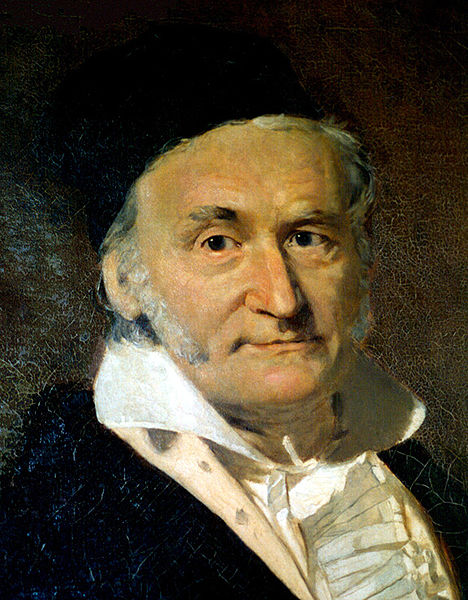
\includegraphics{468px-Carl_Friedrich_Gauss}}

\begin{document}

\maketitle

\tableofcontents

\chapterimage{321px-Euklid2}
\chaptertext{\textbf{Euclide}, en grec ancien \emph{Eukleids} (n vers \textminus 325, mort vers \textminus 265  Alexandrie) est un mathmaticien de la Grce antique ayant probablement vcu en Afrique, auteur des lments, qui sont considrs comme l'un des textes fondateurs des mathmatiques modernes.

Peu d'informations sont connues  propos de la vie d'Euclide. Contemporain d'Archimde (n en \textminus 287 et mort en \textminus 212), il nat vers \textminus 325 et meurt vers \textminus 265, mais, selon le mathmaticien Christian Velpryses, ses dates de naissance et de mort sont inconnues.

Il part en gypte pour y enseigner les mathmatiques sous le rgne de Ptolme I\ier. Il travaille au muse d'Alexandrie et  l'cole de mathmatiques. Entour de ses disciples, il mne de nombreux travaux de recherche.

\smallbreak

\hfill(\textit{Source~:} Wikipdia)}
\chapter{Divisibilit, PGCD, PPCM}

\section{Divisibilit dans $\N$}

\subsection{Diviseurs}

\begin{definition}
Soient $d$ et $n$ des entiers naturels. On dit que $d$ divise (\emph{ou} \og est un diviseur de\fg{} \emph{ou} \og est divisible par\fg{}) $n$ s'il existe $q \in \N$ tel que $n = dq$.
\end{definition}

\begin{exemple}
Le nombre $385$ est divisible par $5$ car $385 = 5 \times 77$.
\end{exemple}

\begin{remarques}
\begin{sousremarques}
    \item Le nombre $1$ divise tous les nombres. C'est le seul  avoir cette proprit.
    \item Un nombre $n$ est toujours divisible par $n$.
    \item Le seul nombre divisible par $0$ est $0$ lui-mme.
    \item Le nombre $0$ est divisible par tous les nombres. C'est le seul  avoir cette proprit.
\end{sousremarques}
\end{remarques}

\begin{definition}
Soit $n$ un entier naturel. L'ensemble des diviseurs de $n$, not $\ensdiv(n)$, est l'ensemble des $d \in \N$ qui divisent $n$.
\end{definition}

\begin{exemple}
On a $\ensdiv{385} = \ens{1,5,7,11,35,55,77,385}$. On verra plus tard une mthode simple pour justifier rigoureusement cela.
\end{exemple}

\begin{proprietes}
\begin{sousproprietes}
    \item Si $dd'$ divise $n$, alors $d$ divise $n$ et $d'$ divise $n$.
    \item Si $n \neq 0$ et si $d$ divise $n$, alors $1 \leq d \leq n$.
    \item Si $d$ divise $b$ et si $c$ divise $d$, alors $c$ divise $n$.
    \item Si $d$ divise $n$ et $m$, alors $d$ divise $un+vm$ pour tous les entiers $u$ et $v$.
\end{sousproprietes}
\end{proprietes}

\subsection{Multiples}

\begin{definition}
Soient $n$ et $m$ deux entiers naturels. On dit que $m$ est un multiple de $n$ s'il existe $k \in \N$ tel que $m = kn$.
\end{definition}

\begin{exemple}
Le nombre $42$ est un multiple de $6$ car $42 = 6 \times 7$.
\end{exemple}

\begin{propriete}
$m$ est un multiple de $n$ si et seulement si $n$ divise $m$.
\end{propriete}

\section{Division euclidienne dans $\N$}

\begin{theoreme}
Soient $a$ et $b$ deux entiers naturels. Si $b \neq 0$, alors il existe un unique couple $(q,r)$ tel que
\[a = bq + r \quad \text{avec $0 \leq r < b$.}\]
\end{theoreme}

\begin{demonstration}
Puisque $b$ est non nul, il existe $q$ tel que $bq \leq a < b(q+1)$. On pose $r = a-bq$ et on a le rsultat voulu.
\end{demonstration}

\begin{exemple}
Trouvons la division euclidienne de $314$ par $78$. On a $2 \times 78 = 156$, $3 \times 78 = 234$, $4 \times 78 = 312$ et $5 \times 78 = 390$ et donc $312 \leq 314 < 390$, d'o $q = 4$ et $r = 314-312 = 2$. La division euclidienne est donc $314 = 78 \times 4 + 2$.
\end{exemple}

\begin{definition}
L'entier $q$ est appel le \definir{quotient} de la division euclidienne et l'entier $r$ est le \definir{reste} de la division euclidienne.
\end{definition}

\begin{proprietes}
\begin{sousproprietes}
    \item Le nombre $b$ divise $a$ si et seulement si $r=0$.
    \item Si $b < a$, alors $q=0$ et $r=b$.
    \item Tout entier $n$ positif s'crit sous la forme $bq+r$ avec $r=0$, $r=1$, \dots{} ou $r=n-1$.
\end{sousproprietes}
\end{proprietes}

\section{Diviseurs communs  deux entiers}

\subsection{Dfinition}

\begin{definition}
Si $a$ et $b$ sont deux entiers naturels, on note $\ensdiv{a,b}$ l'ensemble des diviseurs communs  $a$ et $b$.
\end{definition}

\begin{exemple}
On a $\ensdiv{12,8} = \ens{1,2,4}$.
\end{exemple}

\begin{proprietes}\label{ref:propr:ensdiv.commun}
\begin{sousproprietes}
    \item Si $a$ et $b$ sont deux entiers naturels, $\ensdiv{a,b} = \ensdiv{a} \cap \ensdiv{b}$.
    \item On a toujours $1 \in \ensdiv{a,b}$.
    \item Si $d \in \ensdiv{a,b}$ avec $a \neq 0$ et $b \neq 0$, alors $d \leq \max(a,b)$.
    \item $\ensdiv{a,0} = \ensdiv{a}$.
\end{sousproprietes}
\end{proprietes}

\begin{theoreme}
Si $a$ et $b$ ne sont pas tous nuls, l'ensemble $\ensdiv{a,b}$ a un plus grand lment $d$ que l'on appelle le \definir{pgcd} (plus grand diviseur commun) de $a$ et $b$.
\end{theoreme}

\begin{demonstration}
Si $a = 0$ et $b \neq 0$, on a $\ensdiv{a,b} = \ensdiv{a,0} = \ensdiv{a}$ et donc $d = a$ convient~; si $b = 0$ et $a \neq 0$, de mme $d = b$ convient. Si $a \neq 0$ et $b \neq 0$, alors, d'aprs la proprit~\ref{ref:propr:ensdiv.commun}, l'ensemble $\ensdiv{a,b}$ est non vide et est major~; il possde donc un plus grand lment $d$.
\end{demonstration}

\begin{remarque}
Le pgcd de $0$ et $0$ n'est pas dfini car $\ensdiv{0,0} = \ensdiv{0} = \N$ n'a pas de plus grand lment.
\end{remarque}

\subsection{Algorithme d'Euclide}

L'algorithme d'Euclide permet de trouver le pgcd de deux nombres. L'ide est de construire une suite d'entiers $r_i$ tels que
\[\ensdiv{a,b} = \ensdiv{b,r_1} = \ensdiv{r_1,r_2} = \dots \ensdiv{r_n,0} = \ensdiv{r_n}\]
 auquel cas $r_n$ sera le plus grand diviseur commun  $a$ et $b$.

\subsubsection{Ensemble des diviseurs et division euclidiennes}

\begin{lemme}
Soient $a$ et $b$ deux entiers naturels non nuls. Si on peut crire $a = bq + r$ avec $q,r \in \N$ (on ne suppose pas \emph{a priori} que $0 \leq r < b$), alors $\ensdiv{a,b} = \ensdiv{b,r}$.
\end{lemme}

\begin{demonstration}
Si $d \in \ensdiv{a,b}$, alors $d$ divise $a$ et $b$ donc divise $a-bq = r$ et donc $d \in \ensdiv{b,r}$. Rciproquement, si $d \in \ensdiv{b,r}$, alors $d$ divise $bq+r = a$ et donc $d \in \ensdiv{a,b}$.
\end{demonstration}

\subsubsection{Divisions euclidiennes successives}

\begin{theoreme}[Algorithme d'Euclide]
Soient $a$ et $b$ deux entiers naturels non nuls. On crit les divisions euclidiennes successives
\begin{alignat*}{3}
& a=bq_1+r_1 &\quad& \text{avec $0 \leq r_1 < b$} \\
& b=r_1q_2+r_2 &\quad& \text{avec $0 \leq r_2 < r_1$}&\quad& \text{(possible si $r_1 \neq 0$)} \\
& r_1=r_2q_3+r_3 &\quad& \text{avec $0 \leq r_3 < r_2$}&\quad& \text{(possible si $r_2 \neq 0$)}\\
& \dots
\end{alignat*}
Il existe un rang $n \in \N^*$ tel que $r_n = 0$.
\end{theoreme}

\begin{demonstration}
Il suffit de remarquer que s'il n'existait pas de rang $n$ tel que $r_n = 0$, alors la suite $(r_i)$ serait une suite strictement dcroissante d'entiers naturels, ce qui est absurde.
\end{demonstration}

\subsubsection{Consquence pour le pgcd}

\begin{corollaire}
Soient $a$ et $b$ deux entiers naturels non tous nuls. Le pgcd de $a$ et $b$ est l'unique entier $d$ tel que $\ensdiv{a,b} = \ensdiv{d}$.
\end{corollaire}

\begin{demonstration}
C'est juste une reformulation de l'algorithme d'Euclide~: $\ensdiv{a,b} = \ensdiv{b,r_1} = \dots = \ensdiv{r_n,0} = \ensdiv{r_n}$ et donc le plus grand lment de $\ensdiv{a,b}$ est $d = r_n$.
\end{demonstration}

\subsection{Relation de Bzout}

\begin{theoreme}
Soient $a$ et $b$ deux entiers naturels non tous nuls. Un entier $d$ est le pgcd de $a$ et $b$ si et seulement si $d$ divise $a$ et $b$ et s'il existe $u$ et $v$ tels que
\[au+bv=d\]
\end{theoreme}

\begin{demonstration}
$\impliedby$~: Supposons que $d$ divise $a$ et $b$ et qu'on puisse crire $d=au+bv$. Si $c$ est un diviseur commun  $a$ et $b$, alors $c$ divise $au+bv = d$~; autrement dit, tout lment de $\ensdiv{a,b}$ divise $d$~; on en dduit que le pgcd de $a$ et $b$ est $\leq d$. Puisqu'il est aussi $\geq d$ car $d \in \ensdiv{a,b}$ , on conclut que $d$ est le pgcd de $a$ et $b$;

$\implies$~: Soit $d$ le pgcd de $a$ et $b$~; il est vident que $d$ divise $a$ et $b$~; montrons l'existence de $u$ et $v$. On utilise l'algorithme d'Euclide~:
\begin{align*}
& a=bq_1+r_1 \quad \text{avec $0 \leq r_1 < b$} \\
& b=r_1q_2+r_2 \quad \text{avec $0 \leq r_2 < r_1$ (possible si $r_1 \neq 0$)} \\
& r_1=r_2q_3+r_3 \quad \text{avec $0 \leq r_3 < r_2$ (possible si $r_2 \neq 0$)} \\
& \dots \\
& r_{n-1} = r_n q_{n+1} + 0
\end{align*}
On a $d = r_{n}$. Montrons par rcurrence sur $i \leq n$ que l'on peut crire $r_i = a u_i + b v_i$. On a
\[r_1 = a - bq_1 \quad{et donc} u_1 = 1 \quad \text{et} \quad v_1 = -q_1.\]
Supposons que $r_i = au_i+bv_i$ avec $i < n$ et montrons que $r_{i+1} = au_{i+1} + bv_{i+1}$. On a
\[r_{i+1} = r_{i-1} - q_{i+1} r_i = a u_{i-1} + b v_{i-1} - q_{i+1} (a u_{i} + b v_{i}) = a (u_{i-1} - q_{i+1} u_{i}) + b(v_{i-1} - q_{i+1} v_{i}),\]
et donc le choix $u_{i+1} = u_{i-1} - q_{i+1} u_{i}$ et $v_{i+1} = v_{i-1} - q_{i+1} v_{i}$ convient. En particulier, pour $i=n$, on obtient, en posant $u_n = u$ et $v_n = v$,
\[d = r_n = a u_n + b v_n = au + bv.\]
La dmonstration est termine.
\end{demonstration}

\section{Proprits du pgcd}

\subsection{Entiers premiers entre eux}

\begin{definition}
Deux entiers naturels non nuls $a$ et $b$ sont dit premiers entre eux si et seulement si leur pgcd vaut $1$.
\end{definition}

\begin{lemme}[lemme de Gauss]
Soient $a$, $b$ et $c$ des entiers naturels non nuls. Si $a$ divise $bc$ avec $a$ et $b$ premiers entre eux, alors $a$ divise $b$ ou $a$ divise $c$.
\end{lemme}

\begin{demonstration}
Puisque $a$ et $b$ sont premiers entre eux, il existe $u$ et $v$ tels que $au+bv=1$~; en multipliant par $c$, on obtient $acu+bcu=c$. Puisque $a$ divise $bc$, on en dduit que $a$ divise $c$.
\end{demonstration}

\begin{corollaire}
Soient $a$ et $b$ deux entiers naturels premiers entre eux. Si $a$ et $b$ divisent $n$, alors $ab$ divise $n$.
\end{corollaire}

\begin{demonstration}
Puisque $a$ divise $n$, on peut crire $n = aq$~; puisque $b$ divise $n$, il divise $aq$ et puisque $a$ et $b$ sont premiers entre eux, $b$ divise $q$ et donc on peut crire $q = bk$ et donc $n = abk$, ce qui montre que $ab$ divise $n$.
\end{demonstration}

\subsection{Mutliplicativit}

\begin{propriete}
Soient $a$, $b$ et $c$ trois entiers naturels non nuls et $d$ le pgcd de $a$ et $b$. Le pgcd de $ac$ et $bc$ est $dc$.
\end{propriete}

\begin{demonstration}
Il est vident que $dc$ est un diviseur commun  $ac$ et $bc$. C'est le pgcd car on peut crire $au+bv=d$ et donc $(ac)u+(bc)v = dc$.
\end{demonstration}

\section{Notion de ppcm}

\subsection{Dfinition}

L'ensemble des multiples communs  $a$ et $b$ est non vide (il contient $ab$) et minor par $\min(a,b)$~; il possde donc un plus petit lment, not $m$ et appel le \definir{ppcm} (plus petit commun multiple) de $a$ et $b$.

\subsection{Lien avec le pgcd}

\begin{propriete}
Soient $a$ et $b$ deux entiers naturels non nuls, $d$ leur pgcd et $m$ leur ppcm.
\begin{sousproprietes}
    \item $md = ab$.
    \item Tout multiple commun  $a$ et $b$ est multiple de $m$.
\end{sousproprietes}
\end{propriete}

\begin{demonstration}
\begin{sousdemonstration}
    \item Notons tout d'abord que $m' = \frac{ab}{d}$ est un multiple commun  $a$ et $b$~; en effet, si on pose $a = da'$ et $b = db'$, on a $m' = a'b$ donc $m'$ est un multiple de $b$ et $m' = ab'$ donc $m'$ est un multiple de $a$.

Reste  montrer que $m' = m$. Soit $\mu$ un multiple quelconque de $a$ et $b$~; puisque $\mu$ est un multiple commun  $a$ et $b$ donc on peut crire $\mu = ak$ et $\mu = bk'$. On a donc $a'dk = b'dk'$ d'o $a'k = b'k'$~; puisque $a'$ et $b'$ sont premiers entre eux (consquence de la relation de Bzout), on en dduit que $a'$ divise $k'$ et donc $k' = a' k''$~; ainsi, $m = a'b'd k'' = m' k''$ et donc $m' \leq \mu$, ce qui montre que $\mu$ est multiple de $m'$~; le multiple $\mu$ tant arbitraire, on en dduit que $m'$ est le ppcm de $a$ et $b$.
    \item Comme on vient de le voir, tout multiple de $a$ et $b$ est multiple de $m' = m$, d'o le rsultat.
\end{sousdemonstration}
\end{demonstration}

\modeexercice
\section{Exercices et problmes}

\begin{listeexercices}

\subsection{Diviseurs et multiples}

\begin{exercice}
crire la liste des diviseurs des nombres suivants.
\[13, \quad 56, \quad 198, \quad 6754, \quad 12553.\]
\end{exercice}

\begin{exercice}
crire la liste des multiples $\leq 200$ des nombres suivants.
\[7, \quad 36, \quad 27, \quad 89, \quad 101, \quad 59, \quad 13.\]
\end{exercice}

\begin{exercice}
Si $a \in \N$, montrer que $a(a-1)$ est pair et que $a(a^2-1)$ est divisible par $3$.
\end{exercice}

\begin{exercice}\difficulte{1}
Dterminer les entiers $n$ tels que $u_n = n^2-3n+6$ soit un multiple de $n$.
\end{exercice}

\subsection{Division euclidienne}

\begin{exercice}
Effectuer les divisions euclidiennes de $a$ par $b$ dans les cas suivants.
\begin{multicols}{2}
\begin{questions}
    \item $a = 87$ et $b = 5$.
    \item $a = 454$ et $b = 33$.
    \item $a = 765$ et $b = 890$.
    \item $a = 8997$ et $b = 654$.
\end{questions}
\end{multicols}
\end{exercice}

\begin{exercice}
On effectue la division euclidienne de $a = 124$ par un entier $b$ et on trouve un quotient $q$ un reste gal  $r = 9$. Quelles sont les valeurs possibles de $b$ et $q$~?
\end{exercice}

\begin{exercice}
On crit $a = bq+r$ la division euclidienne de $a$ par $b$. Quelle est la division euclidienne de $a+1$ par $b$~? de $a+kb$ par $b$~?
\end{exercice}

\subsection{Algorithme d'Euclide, pgcd}

\begin{exercice}\label{exo:divisibilite:algo.euclide}
En utilisant l'algorithme d'Euclide, calculer le pgcd des nombres $a$ et $b$ suivants.
\begin{multicols}{2}
\begin{questions}
    \item $a = 87$ et $b = 5$.
    \item $a = 454$ et $b = 33$.
    \item $a = 765$ et $b = 890$.
    \item $a = 8997$ et $b = 654$.
\end{questions}
\end{multicols}
\end{exercice}

\begin{exercice}
On effectue l'algorithme d'Euclide pour des nombres $a$ et $b$ et on trouve pour pgcd $r_4 = 39$ et comme suite de quotients successifs $q_1 = 1$, $q_2 = 5$, $q_3 = 1$, $q_4 = 6$ et $q_5 = 2$. Quelle est la valeur de $a$ et $b$~?
\end{exercice}

\begin{exercice}\difficulte{1}
Trouver des entiers naturels tels que $a+b=72$ et $\pgcd(a,b) = 8$.
\end{exercice}

\begin{exercice}
Reprendre les entiers de l'exercice~\ref{exo:divisibilite:algo.euclide} et crire une relation de la forme $au+bv=d$ o $d = \pgcd(a,b)$.
\end{exercice}

\subsection{ppcm}

\begin{exercice}
Reprendre les entiers de l'exercice~\ref{exo:divisibilite:algo.euclide} et trouver leur ppcm.
\end{exercice}

\begin{exercice}
Trouver deux entiers naturels $a$ et $b$ tels que $\pgcd(a,b) = 24$ et $\ppcm(a,b) = 2160$.
\end{exercice}

\begin{exercice}
Vrifier que
\begin{align*}
\ppcm(1,2,3,4)
& = 2\sin\tfrac{\pi}{2} \times 2\sin\tfrac{\pi}{3} \times 2\sin\tfrac{2\pi}{3} \\
& \qquad \times 2\sin\tfrac{\pi}{4} \times 2\sin\tfrac{3\pi}{4}
\end{align*}
(On fait le produit sur les $2\sin\tfrac{k\pi}{n}$ avec $k$ et $n$ premiers entre eux pour $n = 2$, $3$ ou $4$.)
\end{exercice}

\end{listeexercices}
\modenormal

\chapterimage{468px-Carl_Friedrich_Gauss}
\chaptertext{\textbf{Johann Carl Friedrich Gauss} (30 avril 1777 -- 23 fvrier 1855) est un mathmaticien, astronome et physicien allemand. Dot d'un grand gnie, il a apport de trs importantes contributions  ces trois sciences. Surnomm \og le prince des mathmaticiens\fg{}, il est considr comme l'un des plus grands mathmaticiens de tous les temps.

La qualit extraordinaire de ses travaux scientifiques tait dj reconnue par ses contemporains. Ds 1856, le roi de Hanovre fit graver des pices commmoratives avec l'image de Gauss et l'inscription Mathematicorum Principi (\og prince des mathmaticiens\fg{} en latin). Gauss n'ayant publi qu'une partie infime de ses dcouvertes, la postrit dcouvrit la profondeur et l'tendue de son \oe uvre uniquement lorsque son journal intime, publi en 1898, fut dcouvert et exploit.

Considr par beaucoup comme distant et austre, Gauss ne travailla jamais comme professeur de mathmatiques, dtestait enseigner et collabora rarement avec d'autres mathmaticiens. Malgr cela, plusieurs de ses tudiants devinrent de grands mathmaticiens, notamment Richard Dedekind et Bernhard Riemann.

Gauss tait profondment pieux et conservateur. Il soutint la monarchie et s'opposa  Napolon qu'il vit comme un semeur de rvolution.

\smallbreak

\hfill(\textit{Source~:} Wikipdia)}
\chapter{Nombres premiers}

\section{Dfinitions}

\begin{definition}
Un nombre entier $p \geq 2$ est \definir{premier} s'il divisible uniquement par $1$ et par lui-mme.
\end{definition}

\begin{remarque}
Noter que $1$ n'est pas un nombre premier. La raison est que c'est le seul nombre qui divise tous les autres. Les nombres premiers ont une proprit moins forte~: tout nombre $\geq 2$ est divisible par un nombre premier.
\end{remarque}

\begin{exemples}
\begin{sousexemples}
    \item Les premiers nombres premiers sont~: $2$, $3$, $5$, $7$, $11$, $13$, $17$, $19$, $23$, $29$, $31$, $37$, $41$, $43$, $47$, $53$, $59$, $61$, $67$, $71$, $73$, $79$, $83$, $89$, $97$, etc. Il y a une infinit de nombre premiers, comme on le verra dans le corollaire~\ref{theoreme:euclide}.
    \item L'un des nombres premiers les plus grands est $2^{43112609}-1$ (c'est un nombre premier de Mersenne, c'est--dire un nombre premier de la forme $2^k-1$).
\end{sousexemples}
\end{exemples}

\section{Proprits de divisibilit des nombres premiers}

\begin{lemme}[Lemme de Gauss]\label{lemme.Gauss}
Un nombre $p \geq 2$ est premier si et seulement si $p \mid ab \implies p \mid a \text{ ou } p \mid b$.
\end{lemme}

\begin{demonstration}
Soit $p \geq 2$ vrifiant $p \mid ab \implies p \mid a \text{ ou } p \mid b$. Si $d$ divise $p$, alors on peut crire $p = dq$ et donc $p \mid d$ ou $p \mid q$. Dans le premier cas, $d = p$, et dans le second, $d = 1$, ce qui montre que les seuls diviseurs de $p$ sont $1$ et $p$.

Rciproquement, considrons un nombre premier $p$ et supposons que $p \mid ab$. Le pgcd de $p$ et $a$ est soit $1$ soit $p$~; si ce n'est pas $p$, alors on peut crire $pu+av=1$ et donc $pub + abv = b$ c'est--dire que $p$ divise $b$ vu que $p \mid ab$.
\end{demonstration}

\section{Dcomposition en facteurs premiers}

\subsection{Thorme fondamental}

\begin{theoreme}[Thorme fondamental de l'arithmtique]\label{theoreme:TFA}
Tout nombre premier $n \geq 2$ s'crit comme produit de nombres premiers.
\end{theoreme}

\begin{demonstration}
Pour l'existence, on procde par rcurrence. Si $n = 2$, c'est vident car $n$ est premier. Si $n \geq 3$ n'est pas premier, alors on peut l'crire sous la forme $n = dq$ avec $1 < d < n$ et $1 < q < n$. Par hypothse de rcurrence, $d$ et $q$ sont des produits de nombres premiers et donc il en est de mme de $n$.

Montrons l'unicit en utilisant le lemme de Gauss (lemme~\ref{lemme.Gauss}). Si $n = p_1 \dots p_r = q_1 \dots q_s$ avec les $p_i$ et les $q_j$ premiers, alors, puisque $p_1 \mid q_1 \dots q_s$, $p_1$ divise un des $q_j$, disons $q_1$ (quitte  r-indexer les $q_j$ si ncessaire); ces deux nombres tant premiers, on en dduit que $p_1 = q_1$ et donc on obtient $p_2 \dots p_r = q_2 \dots q_s$. Le mme raisonnement fournit $p_2 = q_2$ (quitte  rindexer les $q_j$ au besoin), etc. Finalement, $r = s$ et $p_i = q_i$ pour tout $i$.
\end{demonstration}

Tout entier $n \geq 2$ s'crit donc de manire unique sous la forme $n = p^{\alpha_1} \dots p_r^{\alpha_r}$ avec les $p_i$ des nombres premiers distincts et les $\alpha_i$ des entiers $\geq 1$.

\begin{exemples}
\begin{sousexemples}
    \item $24 = 2^3 \times 3$
    \item $255 = 3 \times 5 \times 17$
    \item $663 = 7 \times 13 \times 17$
\end{sousexemples}
\end{exemples}

\subsection{Consquences}

Soit $n \geq 2$ qu'on crit sous la forme $n = p^{\alpha_1} \dots p_r^{\alpha_r}$ avec les $p_i$ des nombres premiers deux  deux distincts. On pose $v_{p_i}(n) = \alpha_i$ et $v_p(n)=0$ si $p$ n'est pas l'un des $p_i$. Ceci permet d'crire
\[n = \prod_{\text{$p$ premier}}{p^{v_p(n)}}.\]

\begin{corollaire}[Calcul du pgcd]
\[\pgcd(m,n) = \prod_{\text{$p$ premier}}{p^{\min(v_p(n),v_p(m))}}\]
\end{corollaire}

\begin{exemple}
Le pgcd de $24 = 2^3 \times 3$ et $306 = 2 \times 3^2 \times 17$ est $2^1 \times 3^1 \times 17^0 = 6$.
\end{exemple}

\begin{corollaire}[Calcul du ppcm]
\[\ppcm(m,n) = \prod_{\text{$p$ premier}}{p^{\max(v_p(n),v_p(m))}}\]
\end{corollaire}

\begin{exemple}
Le ppcm de $24 = 2^3 \times 3$ et $306 = 2 \times 3^2 \times 17$ est $2^3 \times 3^2 \times 17^1 = 1224$.
\end{exemple}

\section{Quelques proprits de l'ensemble des nombres premiers}

\begin{theoreme}[Thorme d'Euclide]\label{theoreme:euclide}
Il existe une infinit de nombre premiers.
\end{theoreme}

\begin{demonstration}
Considrons un ensemble fini $\{p_1,\dots,p_r\}$ de nombre premiers et posons $N = p_1 \dots p_r + 1$. Le nombre $N$ est $\geq 2$ donc est divisible au moins par un nombre premier $q$, mais ce nombre premier ne peut tre l'un des $p_i$ car aucun des $p_i$ ne divise $N$ (dans le cas contraire, ce $p_i$ diviserait $1$). Ceci montre qu' chaque fois qu'on a un nombre fini de nombres premiers, on peut en construire un autre~; c'est le rsultat voulu.
\end{demonstration}


\modeexercice % entre en mode exercice
\section{Exercices et problmes}

\begin{listeexercices}

\subsection{Nombres premiers}

Pour les deux exercices suivants, dire si les nombres donns sont premiers.

\begin{exercice}
$353$~; $457$~; $101$~; $89$~; $113$.
\end{exercice}

\begin{exercice}
$1453$~; $1267$~; $7651$~; $1789$.
\end{exercice}

\begin{exercice}
Les nombres $1$, $11$, $111$, $1111$, $11111$, $111111$ sont-ils premiers~?
\end{exercice}

\begin{exercice}
crire la liste des nombres premiers compris entre 100 et 200.
\end{exercice}

\subsection{Dcompositions en facteurs premiers}

Pour les deux exercices suivants, trouver la dcomposition en facteurs premiers des nombres donns. En dduire l'ensemble des diviseurs de chacun des nombres

\begin{exercice}
$567$~; $546$~; $897$~; $564$~; $890$.
\end{exercice}

\begin{exercice}
$4637$~; $3560$~; $9884$~; $2010$.
\end{exercice}

\begin{exercice}\difficulte{1}
On pose $n = 900\dots 0$. Combien faut-il de zros pour que $b$ admette $108$ diviseurs (positifs)~?
\end{exercice}

\begin{exercice}
Comment reconnat-on sur la dcomposition en facteurs premiers de $n$ que $n$ est un carr~?
\end{exercice}

\begin{exercice}
On pose $u_0 = 2$ et $u_{n+1} = 1 + \prod_{\text{$p$ premier}}{p^{v_p(u_n)}}$.
\begin{questions}
    \item O a-t-on dj rencontr cette suite~?
    \item Calculer $u_1$, $u_2$, $u_3$, $u_4$, $u_5$.
\end{questions}
\end{exercice}

\begin{exercice}
\begin{questions}
    \item Montrer que si $n$ et $m$ sont deux nombres premiers entre eux tels que $nm$ est un carr, alors $n$ et $m$ sont des carrs~?
    \item Le rsultat prcdent reste-t-il valable pour des puissances $k$-imes avec $k \geq 2$~?
\end{questions}
\end{exercice}

\subsection{Pgcd et ppcm}

\begin{exercice}
Pour chacun des couples suivants, trouver leur pgcd et leur ppcm en utilisant la dcomposition en facteurs premiers.
\[(1236,764)~; \quad (784,8760)~; \quad (765,875).\]
\end{exercice}

\subsection{Ensemble des nombres premiers}

\begin{exercice}
Dmontrer que la suite $((n+2)!+k)_{2 \leq k \leq n+1}$ est une suite de $n$ nombres tous non premiers.
\end{exercice}

\begin{exercice}\difficulte{1}
Montrer qu'il existe une infinit de nombre premiers de la forme $4k-1$.
\end{exercice}

\begin{exercice}\difficulte{2}
Montrer qu'il existe une infinit de nombre premiers de la forme $4k+1$.
\end{exercice}

\subsection{Exercices de recherche}

\begin{exercice}\difficulte{3}
Montrer que si $p$ est premier et si $a$ est premier  $p$, alors $a^{p-1}-1$ est divisible par $p$.
\end{exercice}

\begin{exercice}\difficulte{2}
Soit $n$ un nombre tel que, pour tout $a$ premier  $p$, le nombre $a^{p-1} - 1$ est divisible par $n$. Est-ce que $n$ est premier~?
\end{exercice}

\begin{exercice}\difficulte{3}
Montrer que $p$ est premier si et seulement si $(p-1)!+1$ est divisible par $p$.
\end{exercice}

\end{listeexercices}
\modenormal % restaure les dfinitions de sections, sous-sections, etc;

\end{document}
